\chapter{Realisation}
This chapter details all the information about the realisation of Smart Sponsor. After looking at the chosen programming languages, framework, and IDE, the implementation follows. Design decisions of some impact are expanded upon. Finally, the project will be analyzed from a performance aspect. The conclusions following this analysis will be detailed in the next chapter. The repository of the final code can be found here:
\url{https://github.com/ChristophSchrieverRWTH/Smart-Sponsor-v3}
\section{Tool Selection}
Smart Sponsor's development was separated into the front- and back-end development. The back-end uses a blockchain for its' data storage. Due to familiarity with curly-bracket languages and the availability of development tools the blockchain of choice was "Ethereum" using its appended programming language "Solidity." The chosen development environment was "Truffle"\cite{truffle}, as it supports unit tests using the "Mocha" testing framework and "Chai" and easy access to a test blockchain. For most of the development the test blockchain "Ganache"\cite{truffle} was used. For some parts, the browser-based IDE Remix\cite{remix} was used. The back end of the server was run using Node. The full list of packages can be found in the repository.\\
The front end was developed using "Visual Studio Code" as its IDE. The user interface was created using "Bootstrap" and "React." React allows for creating a single-page application and allows for the grouping of HTML elements into components. These components give more structure to the code. The front-end logic was implemented using "JavaScript." Front-end access to the blockchain runs through the browser extension "MetaMask"\cite{meta}.\\
The version control of Smart Sponsor was secured using GitHub.
\section{Back-End Implementation}
The back-end segment will deal with the Solidity code and some of the unit tests. Most design decisions here deal with performance or security.
\subsection{Verification of Conditions}
As the verification of conditions is one of the fundamental concepts of Smart Sponsor, its implementation stands as the foundation. In this way, the verification can also be seen as an axiom to any of the transactions of the banking system or Smart Sponsor. The smart contract needs to allow adding and checking certificates, but it also needs to accommodate certificates expiring. The process of creating a certificate is detailed in algorithm 1. Checking a certificate requires recalculating the hash. Updating which certificates have expired works as described in algorithm 2. Both functions that write on the blockchain are restricted to being useable by the owner only. This security is secured by OpenZeppelin's "Ownable" smart contract\cite{Zeppelin}.\\
\begin{algorithm}
\caption{Creating a certificate}\label{alg:create}
\begin{algorithmic}
\Require $message.sender = Verification.owner$
\Require $condition \neq null$
\Require $user \neq null$
\Require $expiryDate \neq null$
\State $concat \gets concatenate(condition, user)$ 
\State $certificate \gets hash(concat)$
\If{$certificateTable[certificate] = false$}
    \State $certificateTable[certificate] \gets true $
\EndIf
\State $expiryTable[certificate] \gets expiryDate$
\end{algorithmic}
\end{algorithm}
\\
After sending a request to get a condition verified the personnel or program responsible for determining if a condition is fulfilled would create a certificate for the address of the user who made this request.\\
The central piece of adding and verifying certificates in the verification process is Solidity's built-in hashing algorithm "keccak256". In practice, this function would get called by the third-party verification service. The keccak256 function belongs to the same family as all the SHA-3 functions do. Apart from being irreversible it also boasts security against collision attacks and length extension attacks. The input we give is a string that results from the concatenation of the user's address and the string representing the condition e.g. "\emph{Younger than 23 years old.}"\\
To concatenate strings the \emph{abi.encode} and \emph{abi.encodePacked} functions exist as default functions given by Solidity. The main difference is in how strings smaller than 32 bytes are handled. Abi.encode always pads up to 32 bytes. The latter is more space-efficient but as it does not pad empty bits the resulting string might run into collision danger:
\begin{equation*}
    keccak(AAA, BBB) \Longleftrightarrow keccak(AA, ABBB)
\end{equation*}
Still, this more compact version is usable without a problem, as we know the length of one of our input strings. An Ethereum address is always 20 bytes large. This represents 40 hex characters. Therefore it is always clear where the address ends and where the condition string starts.\\
\begin{algorithm}
\caption{Expiry of certificates}\label{alg:update}
\begin{algorithmic}
\Require $message.sender = Verification.owner$
\State $now = block.timestamp$
\ForEach{$certificate \in certificateTable$}
\If{$expiryTable[certificate] < now$}
\State $certificateTable[certificate] \gets false$
\EndIf
\EndFor
\end{algorithmic}
\end{algorithm}
\\
With the hashing algorithm established, the subject of expiry dates remains. Solidity's internal representation of time relies on the timestamp of the block that is currently being mined. While Ethereum uses the UNIX timestamp to denote this time, it can not be guaranteed that all computers are in agreement with what that currently is. This small discrepancy should only become a problem if enough members of the network create a false consensus on what the current timestamp is. At worst this would cause certificates to expire prematurely which - while a nuisance - does not pose a security threat. How long a certificate should be set valid depends on the type of certificate. Especially time-sensitive conditions like those about age or expiry of documents are to be treated carefully. The hashing over conditions is used to increase the privacy of conditions so setting certificates to exact expiration dates might reveal more information than is necessary. The update function needs to be called once a day. This function can only be called by the owner of the contract leading to higher security.\\
\\
In this version of Smart Sponsor, any possible condition is represented through a string. There are no semantic implications given by this string apart from its existence in the database. It would be possible to replace the string with a more complex datatype detailing eligible values for set keys. In this way checking if a condition is fulfilled could be achieved quickly as the possible values for a key are effectively just a lookup. At the same time, this approach limits the possibilities of what can be proven by a certificate which would reduce the applicability of the financial structure outside of Smart Sponsor.\\ 
\\
Another design decision is the question of how granular conditions should be made.
Smart Sponsor's performance increases if conditions are modeled by strings containing delimiters, but to allow users more reusability, both the back-end- and front-end implementations allow for independent condition strings, while not preventing the user from concatenating conditions into a singular string. \\
It is possible to have $n$ conditions all be contained in a single string of length $L = n + n*delimiter$. As the result of the hashing operation is always a 32bytes-string, the length of the input string does not factor into the output. This approach would lead to faster performance as instead of $n$ certificate checks, now only one is necessary. On the other hand, this approach would reduce versatility. Assuming a user is only missing a single certificate out of $m$ conditions this approach would warrant an entirely new certificate leading to bloat in the database and more strain on the user. What kind of certificate to use should be decided on a case-by-case basis. If a certificate is not due to expire soon and can be reused frequently, combining it into a longer string may be advisable. For example: \emph{store=food; fairTrade=true} with ";" working as a delimiter. If delimited strings are used to denote multiple conditions, said string should be made easily available to the public, possibly being denoted by an abbreviation. On the other hand, certificates that express a more fleeting condition like age or enrollment in a certain university should consequently be written as a singular string, also allowing separate expiry dates for separate conditions.\\
\\
The last major design decision deals with the process of certificates expiring. The check for a certificate's expiry date could be done during the lookup in the database. In this way, there are fewer function calls needed to ensure certificates expire. At the same time, this approach slows down any transaction that needs to verify a certificate. For this reason, the choice of an update function was taken. This approach needs either a script or a person to execute this method once per day leading to a marginal increase in effort once a day but allowing faster checking of certificates.

\subsection{Financial Structure}
The underlying financial infrastructure of Smart Sponsor is the key that enables a proactive implementation of condition-based donations. For ease of reference, the currency detailed in this chapter will henceforth be called "Sponsor Coin." Following a brief consideration of existing token norms, all algorithms dealing with transactions are detailed. Algorithm 3 shows the minting process of new currency. After this algorithm 4 briefly introduces the permission concept, after which algorithms 5 and 6 detail the two transaction methods. The mint function is restricted to only the owner of the smart contract using once again OpenZeppelin\cite{Zeppelin}.\\
\\
Looking at the two most common norms for tokens on blockchains i.e. ERC-20 and ERC-721, neither fully encompass what Sponsor Coin enables. Sponsor Coin is a tokenized form of fiat currency. Every coin is equal in value to every other one. While this at first glance seems similar to ERC-20, the fact that Sponsor Coins can hold vastly different conditions makes them incompatible with this lighter norm. Therefore this approach is a lot closer to ERC-721, also known as Non-Fungible-Token than it is to ERC-20. Every coin is fundamentally different from every other coin. Even if no conditions are attached, they are still separated by their ID. All of them sharing the same value of fiat currency is more of a semantic interpretation than an implemented rule. Yet there exists a need for having different transaction functions, one for transactions that attach new conditions and one that does not. Therefore the resulting contract does not follow either norm but it takes a lot of inspiration from ERC-721.\\
\begin{algorithm}
\caption{Minting new currency}\label{alg:mint}
\begin{algorithmic}
\Require $message.sender = bankOwner$
\Require $user \neq null$
\Require $amount \neq 0$
\State $counter \gets 0$
\While{$counter < amount$}
\State $newCoin \gets new$ $coin(coinID, senderCond, receiverCond)$
\State $coinTable[coinID] \gets newCoin$
\State $ownerTable[coinID] \gets user$
\State $permitTable[coinID] \gets null$
\State $coinID \gets coinID + 1$
\State $counter \gets counter + 1$
\EndWhile
\end{algorithmic}
\end{algorithm}
\\
At the start of a Sponsor Coin's life stands the minting process. In practice, this function would get called visiting a bank or a banking website. After transferring an appropriate amount of fiat currency the minting process gets initiated. But the person who paid for a Sponsor Coin does not necessarily have to become the owner of said coin. This functionality could already be seen as a form of payment or get used for concepts such as grants or pocket money. Therefore the minting process should also allow adding conditions.\\
\begin{equation*}
\begin{array}{c}
    mint() \longrightarrow \emph{$User_A$} \longrightarrow attachTransfer(condition) \longrightarrow \emph{$User_B$} \\
    \big\Downarrow \\
    mint(condition) \longrightarrow \emph{$User_B$}
\end{array}
\end{equation*}
This can make the process of getting an empty coin transferred to another person a lot quicker also reducing the number of transactions needed on the blockchain. Still, this feature does not have to be used and is only an optional shortcut. The owner table exists for quick access when checking ownership. The permit table will be expanded upon following algorithm 4.\\
On top of the 0-address not being accessible by default on Ethereum, it also doubles as the place a token might end its life cycle at. This burning of a token is something that is not necessarily desired with Smart Coins as the idea is to have this currency circulate. Nonetheless keeping this design avenue open allows for easier modification in the future.\\
The minting process also dictates how much fiat currency a singular Sponsor Coin represents, though this is not contained in the blockchain. Again there is no right or wrong answer. The less a coin represents, the more effort the user has to put in to buy a product. Also increasing the number of coins needed proportionally increases the number of function calls needed adversely affecting performance. On the other hand, the more a coin represents the unwieldier it ends up. A value along the lines of 5\EUR{} to 10\EUR{} was envisioned while creating donations, but this value would need to be decided on by convention. There are inherent risks of joining the value of Sponsor Coin with the value of fiat currency, as inflation would increase the amount of computing power needed to fulfill transactions, though the ramifications of this fall outside the scope of this chapter.\\
\begin{algorithm}
\caption{Permitting third-party use of currency}\label{alg:permit}
\begin{algorithmic}
\Require $user \neq null$
\Require $targetIDs \neq null$
\ForEach{$coinID \in targetIDs$}
\If{$ownerTable[coinID] = message.sender$}
\State $permitTable[coinID] \gets user$
\EndIf
\EndFor
\end{algorithmic}
\end{algorithm}
\\
This function would be called by a user who wants to permit the usage of their Sponsor Coins to a third party. There are two use cases for this: Wanting to permit another user to use your coins or allowing a smart contract to use your coins.\\
The former allows the third party to use the currency once a certain event has happened. An example of this could be an escrow-based system.\\
The latter is necessary to circumvent a technical limitation inherent to smart contracts. Assume a normal business transaction of goods being exchanged for money e.g. buying a book. How can this moment of exchange be modeled? In reality, the seller might wait for the buyer to transfer the currency, afterward handing over the wares. This approach is very similar to polling. The seller is waiting for the observed state to change. This approach is not as easily implemented on the blockchain though. Sending the Sponsor Coin first and then calling a function dissociates the two causing a risk of fraud or accidental problems on reverts.\\
A safer approach would be for the sponsor smart contract to use the transfer methods provided by the banking system. But to do this the bank needs to know that the sponsor contract has been allowed to use certain Sponsor Coins. This functions similarly to direct debit authorisation. This approach is also widely found in existing norms e.g. ERC-20 and ERC-721. While in theory permissions could be implemented in a transitive manner, Smart Sponsor's implementation allows no more than one permitted address per coin.\\
\begin{algorithm}
\caption{Transferring Smart Coins without new conditions}\label{alg:normal}
\begin{algorithmic}[1]
\Require $user \neq null$
\Require $targetIDs \neq null$
\ForEach{$coinID \in targetIDs$}
\If{$ownerTable[coinID] = message.sender$ \textbf{or}\\ 
\hspace{30pt}$permitTable[coinID] = message.sender$}
\ForEach{$condition \in coinTable[coinID].senderCond$}
\Ensure $verification.checkCertificate(owner[coinID], condition) = true$
\EndFor
\ForEach{$condition \in coinTable[coinID].receiverCond$}
\Ensure $verification.checkCertificate(user, condition) = true$
\EndFor
\State $ownerTable[coinID] \gets user$
\State $permitTable[coinID] \gets null$
\State $coinTable[coinID].senderCond \gets null$
\State $coinTable[coinID].receiverCond \gets null$
\EndIf
\EndFor
\end{algorithmic}
\end{algorithm}
\\
In practice, this function gets called both by users and smart contracts. Only if the sender fulfills all sender conditions and the receiver fulfills all receiver conditions will the transaction succeed. Afterward, this function clears every condition, both sender and receiver, on every coin involved in the transaction for reasons explained in the context of algorithm 6. There are no limitations on what Sponsor Coins can be sent, as long as the user calling this function has permission to use said coins. Any combination of sender conditions and receiver conditions is permissible as long as the owner of the coins fulfills all conditions. If a third party has initiated a transfer it is still the owner who has to meet the conditions to ensure that no abusable loopholes exist.\\
The performance of this function is tied to how many conditions are attached. The implementation of Smart Sponsor is such that it allows all coins to be mutually distinct and achieve maximum variety. On the other hand, if one assumes that Sponsor Coins tend to group into multiple coins that share the same conditions, variety can be traded for faster performance. A way of implementing this more specified function might force all coins to have the same conditions attached. This would speed up the run time by the number of coins, as now all conditions only have to be ascertained once. As Smart Sponsor is a prototype, a more general approach was taken, allowing for arbitrarily complex combinations at the expense of speed. Another possible option could be to hash over all conditions a coin $C_1$ has set and store these temporarily in a variable. Then before checking if the next coin $C_2$ fulfills any conditions, hash over its conditions. Then compare these to the hashes stored so far. If they match skip the verification for this coin. In this case, unlike detailed in the certificate algorithm, it would be of importance to reconsider whether to use \emph{abi.encode} or \emph{abi.encodePacked} as now a risk of collision exists.\\
\begin{algorithm}
\caption{Transferring Smart Coins attaching new conditions}\label{alg:attach}
\begin{algorithmic}[1]
\Require $user \neq null$
\Require $targetIDs \neq null$
\Require $senderConds \neq null $ \textbf{or} $receiverConds \neq null$
\ForEach{$coinID \in targetIDs$}
\If{$ownerTable[coinID] = message.sender$ \textbf{or}\\ 
\hspace{30pt}$permitTable[coinID] = message.sender$}
\ForEach{$condition \in coinTable[coinID].senderCond$}
\Ensure $verification.checkCertificate(owner[coinID], condition) = true$
\EndFor
\ForEach{$condition \in coinTable[coinID].receiverCond$}
\Ensure $verification.checkCertificate(user, condition) = true$
\EndFor
\State $ownerTable[coinID] \gets user$
\State $permitTable[coinID] \gets null$
\State $coinTable[coinID].senderCond \gets senderConds$
\State $coinTable[coinID].receiverCond \gets receiverConds$
\EndIf
\EndFor
\end{algorithmic}
\end{algorithm}
\\
This function gets called when a user or smart contract sends Sponsor Coins and attaches new conditions. This function differs from algorithm 5 in lines 10, 11 and the requirement of conditions in the first place. For existing conditions algorithm 6 behaves like algorithm 5, only allowing the transaction should all conditions be fulfilled. On the other hand, the new conditions do not need to be fulfilled at the moment of the transaction. It is possible to ascertain that the current receiver of a transaction fulfills the Sponsor Coin's new sender conditions, as they will turn to the sender in the future.  This could reduce the chance of currency reaching a dead-end in the wallet of a user that cannot transfer it. At the same time, this slows down the transaction by the number of sender conditions so Smart Sponsor does not implement this in favour of speed.\\
There are two reasons to have algorithm 5 and algorithm 6 separated. The first is Solidity's concept of local memory. During a function call Solidity differentiates between the \emph{memory} and \emph{storage} keywords when storing arrays or other complex data types. \emph{Storage} denotes data being written to the blockchain while \emph{memory} denotes data being written into a variable. While writing to memory is still far quicker than writing into storage, it is still slower than not using those structures in the first place. Algorithm 5 does not have the two condition arrays as parameters, therefore there is no need to deal with these concepts.\\
The second reason lies in flexibility. While both transaction methods are relevant, introducing new conditions is associated with more variables that could be changed. All design decisions that would affect conditions and certificates would also have ramifications on how conditions are implemented in the financial structure. Having this small redundancy of code allows for easier development, though of course it requires debugging and testing for both methods.\\
Therefore the two transfer functions got separated into the quicker algorithm 5 and the slower algorithm 6.\\
\\
A question that arose during development was how long conditions should be attached to Sponsor Coins. Implementing a counter for each condition on each coin is easily doable by using two more arrays on every coin. While this would decrease performance marginally a larger problem exists. As detailed in chapter 3 the design concept behind Sponsor Coins is such that they can be used both for simple transactions as well as conditional transactions like those occurring during a sponsorship. By allowing a condition to persist through more than one transaction the risk of the coin becoming unusable arises. For example, $User_A$ buys a book with a Sponsor Coin carrying the receiver condition \emph{"store=book"} persisting through two transactions. The store that received this currency can now only spend it at bookstores themselves. Furthermore, should conditions denoting a human be attached e.g. $age<22$, this coin will never be usable by the store. Therefore conditions shall not exist for more than one transaction.\\
\\
The process of attaching conditions posed a fundamental design question. \emph{When should conditions be attached?} There are two options, again neither right nor wrong. One can either attach conditions before the transaction or during it. Attaching conditions is always a process that writes on the blockchain, as the conditions must not be changed to upkeep their integrity. But the situations where a user might want to attach conditions to a Sponsor Coin occur mostly in relation to another user or contract. While the user would have the capability to set themselves conditions, this case should be far less common than prescribing how another may use this money. Therefore splitting the transactions and the attaching process would mostly cause more effort for little gain. On top of that, this effort also translates to more calls to the blockchain, again slowing down performance.\\
Attaching conditions at the same time the currency is moved put less strain on the user and the blockchain. The resulting transaction is of course a singular larger transaction. Depending on the implementation of the underlying blockchain this might cause problems like gas in Ethereum's case. As these smart contracts do not have to be uploaded to the standard Ethereum blockchain but might use an enterprise blockchain instead, this should not pose a problem.\\
Finally, attaching conditions beforehand also eliminates the capability to test if the receiver of a transaction would fulfill the new sender conditions. While Smart Coin is not implemented in this way, this design avenue has been left open for future changes.\\
\\
Attaching conditions in the current version utilises strings. Here lies an inherent restriction solidity poses. Solidity has no functionality to ascertain whether a string is an empty string. There exists a workaround using the keccak256 function. By referencing if the hash of the string in question equals the hash of the empty string, a functional, yet time-intensive workaround is possible.\\
While this solution can identify an empty string, it cannot detect white space such as spaces or tabs. Again removing white space from strings is possible in the back end, but performance-wise it is not practical. Therefore Smart Sponsor's implementation demands the front end to deal with empty strings. Even if empty strings should find their way into a list of conditions the system can handle this as long as the verification hands out a certificate over the empty string. This limitation might also be circumvented using other blockchain services than Solidity.
\subsection{Smart Sponsor}
The preceding smart contracts enable a system of transacting currency only when surrounding conditions are fulfilled. While this allows more control over the flow of one's currency, it does not yet help with charitable giving. Smart Sponsor acts as both a middle agent for the donor and the recipient as well as an additional verification step within the transaction. The smart contract needs to allow setting up sponsorships and applying for them. This is a charity-based system and relies on the goodwill of the donor. Therefore inserting another step to ensure the recipient of a sponsorship actually fulfills its conditions is necessary.\\
The user also needs to be informed about the address of the Smart Sponsor smart contract to allow permitting Sponsor Coins. Algorithm 7 details how a sponsorship is set up while algorithm 8 explains how the application process is handled.\\
\begin{algorithm}
\caption{Setting up a new sponsorship}\label{alg:sponsor}
\begin{algorithmic}
\Require $targetIDs \neq null$
\ForEach{$coinID \in targetIDs$}
\Ensure $bank.ownerTable[coinID] = message.sender$
\EndFor \\
$bank.normalTransfer(address(this), targetIDs)$
\State $offerTable[offerID] \gets new$ $offer(message.sender,$\\ 
\hspace{70pt} $senderConds, receiverConds, targetIDs)$
\State $activeTable[offerID] \gets true$
\State $offerID \gets offerID + 1$
\end{algorithmic}
\end{algorithm}
\\
In practice, this function would get called by users. Still, smart contracts can set up a sponsorship as well. This might allow some applications where money could be pooled and then set up for sponsorship. Unlike algorithm 6 it is not required to attach conditions when creating a sponsorship. While this would equate to giving money to whoever wants to apply without conditions attached, allowing this functionality in the back end has no drawbacks. Smart Sponsor can move currency as long as said coins are permitted for use to Smart Sponsor, even though Smart Sponsor is not the owner of those coins. This is necessary to facilitate smoother transactions. Nonetheless, Smart Sponsor requires the donor who sets up a sponsorship to be the actual owner of the donated coins. This ensures the wishes of the owner are enforced. As Smart Sponsor is not the final receiver of the currency there is no need yet to attach the conditions when transferring the coins. Instead, they are saved in an offer structure that the front end will show to users. The "activeTable" is expanded upon in algorithm 8.\\
There exist a few requirements a user has to fulfill to be able to set up a sponsorship. Smart Sponsor is neither an organisation that can prove it deals in certain goods nor an individual that can show a document of identification. Accordingly, it would be difficult for Smart Sponsor to set up certificates for the receiver conditions on the Sponsor Coins it handles. Therefore it is not possible to call algorithm 7 while receiver conditions are attached to a Sponsor Coin as Smart Sponsor cannot fulfill said conditions.\\
Another option to handle this issue would include creating a list of smart contracts or users that are allowed to ignore conditions, so that receiver conditions would not be verified in case the coin is transferred to Smart Sponsor. This could be similar to the classification of non-profit organisations. This approach is implemented easily and only requires a simple test. The major reason not to do this lies within the breach of trust this could cause. By going closer to the concept of an NPO the same risks currently observable might arise. This whole concept stands opposed to the foundation of trust that is enabled by blockchains.\\
This function is not callable if the sponsor smart contract has not been permitted to use the Sponsor Coins to be donated. But when this function reverts it will give the revert reason that algorithm 5 provided. In this context, this might be confusing for a user in the front end. Therefore, a corresponding error message needs to be displayed on the front end, prompting the user to permit the coins.\\
Similarly to algorithm 6, the same problem with empty strings and white space exists. Again, this prompts a solution in the front end, though in this case, a back-end solution would not be as problematic since algorithm 7 is called less frequently.
\begin{algorithm}
\caption{Applying for a sponsorship}\label{alg:applyOffer}
\begin{algorithmic}
\Require $offerID \neq null$
\Require $activeTable[offerID] = true$
\State $offer \gets offerTable[offerID]$
\ForEach{$condition \in offer.senderConds$}
\Ensure $verification.checkCertificate(message.sender,condition) = true$
\EndFor
\If{$offer.senderCond = null$ \textbf{and}\\ 
\hspace{14pt}$offer.receiverCond = null$}\\
\hspace{30pt}$bank.normalTransfer(message.sender, offer.targetIDs)$
\Else\\
\hspace{30pt}$bank.attachTransfer(message.sender, offer.targetIDs,$\\
\hspace{130pt}$offer.senderConds, offer.receiverConds)$
\EndIf
\State $activeTable[offerID] \gets false$
\end{algorithmic}
\end{algorithm}
\\
Usually, this function would get called by users. Smart contracts can also apply for sponsorships assuming they fulfill all conditions, but it seems unlikely they can pass the more personalized sender conditions. First, it has to be ensured that the application a user applies for is still active. If this is not ensured the resulting behaviour would not be easily decipherable for the user, because the revert will be triggered within algorithm 5 or 6. This can either be solved in the front end or the back end, the chosen implementation. As an additional security measure, algorithm 8 checks if the applicant fulfills all the sender conditions specified in the sponsorship. This poses a small loss of performance. But as applications for a sponsorship are far less common than the transactions explained in algorithms 5 and 6 this small loss of performance can be tolerated for the increased security.\\
If this step was omitted, an actor acting in bad faith could take the donation for himself even if he could not use the coins. The result is an unsatisfied donor and a person still in need of a sponsorship. Even if there are no actively harmful users, a mistaken application could still cause this result. By enforcing the conditions being fulfilled when the applicant applies, at least the currency should never hit a cul-de-sac assuming the user spends the currency before his certificates expire.\\
The conditions that need to be checked are the sender conditions, as the applicant will be the future sender when spending the coins for the final utilisation. Depending on whether conditions are attached to a sponsorship or not, the algorithm that transfers the currency changes. Finally setting this sponsorship to inactive ensures no application attempts are made for a sponsorship that has already been claimed. This is a stop in the backend to ensure safe code. To clarify whether a sponsorship is now inactive or not, using \emph{events} native to Solidity can allow for easier synchronisation with the front end. This falls outside the scope of this project.\\
\\
At this point, the blockchain poses a bit of an issue. A blockchain works by mining blocks containing an undefined but finite number of transaction data. For function calls like those specified before algorithm 8, this poses no problem. In these cases, there is never more than one user attempting to initiate a transaction regarding a piece of data e.g. a certificate or a Sponsor Coin.\\
In contrast, the application for a sponsorship is a lot more competitive in nature. In reality, a transaction such as this would be handled in chronological order, ensuring equal chances. On Ethereum on the other hand the users mining the blocks chose what transactions to include. It is therefore possible for $User_B$ who applied after $User_A$ to win the sponsorship if his transaction is packaged into a block mined first. The average time a block needs to be mined is between 12 to 14 seconds. Therefore the ramifications should not be too noticeable. This problem might be mitigated on an enterprise blockchain which removes the competitive nature of mining blocks. Due to the asynchronous nature of the blockchain, $User_B$ might still apply for a sponsorship $User_A$ just received. But first come first serve should be ensured.\\
\\
These algorithms also contain a function writing to the blockchain that gets called from a different contract than the one it was written in. Both the bank smart contract and the sponsor smart contract need to be initialised with references to the verification smart contract. On top of this, the sponsor smart contract also needs to refer to the bank smart contract. Implementation-wise these functions are close to setter functions, though they should only be callable by the owner of the smart contract. This is the reason, the sponsor contract is again using the "Ownable" smart contract provided by OpenZeppelin\cite{Zeppelin}, even though there are no admin interactions with this smart contract.\\
\section{Front-End Implementation}
The front-end part will deal with connecting to the blockchain from a browser and with the flow of information running through the different React components. Most decisions here deal with accessibility and processing data in such a way the back end does not get overwhelmed.\\
\\
The front end acts as the user interface for all subsystems of Smart Sponsor. As done by Royal et al.\cite{royal} it is imperative to make the blockchain as invisible to the user as possible. Still, it is necessary to sign one's transactions and, if using the public Ethereum blockchain, pay Ether to pay for the gas costs associated with said transactions. Making this step possible requires incorporating libraries to make the user's browser act as a node in the blockchain network. To do this, two steps are necessary.\\
By using the web3.js library\cite{web3} collection, it is possible to adjust the browser to allow remote procedure calls to the blockchain. The web3 library also offers development tools for the development of blockchain-based systems. The truffle suite, which helps with the development of smart contracts and their surrounding systems, has a few community-made setups. Most of those come prebuilt with the web3 libraries allowing for easy updating and development.\\
Secondly, it is necessary to accommodate the features a user of a blockchain might want to use. The first one is connecting to a blockchain wallet. This is usually accomplished using the private key of a wallet key pair. This can be done using the browser extension \emph{MetaMask}\cite{meta}. MetaMask also easily allows signing a transaction. Furthermore, MetaMask has a user base of over 21 Million users\cite{metastat}. For all these reasons, the prototype has been developed with the assumption of users utilising MetaMask. Of course, a larger-scale release would need to adapt to the interface used by the users.\\
\\
Since this is a prototype, there exists no need for larger-scale server structures like a REST-API. All data that will be read by users is stored on the blockchain or supplied by the connection to Smart Sponsor's website. A large-scale operation would probably use a normal database on top of the blockchain to provide quickly accessible user data.\\
For ease of development and accessibility, the Smart Sponsor website was designed as a single-page application, or "SPA" for short. One popular framework to enable this is "React." React's core principle is the component. A component is a reusable block of JavaScript code containing its own set of variables called the "State." In this way, they are similar to normal JavaScript functions. Unlike normal JavaScript functions, a component always returns HTML.\\
Fig 4.1. shows the flow of information through the financial structure's part of the website while Fig 4.2. shows the flow of the sponsor's part. The verification's front end is very linear and does not require such a structure.\\
\begin{figure}[H]
    \centering
    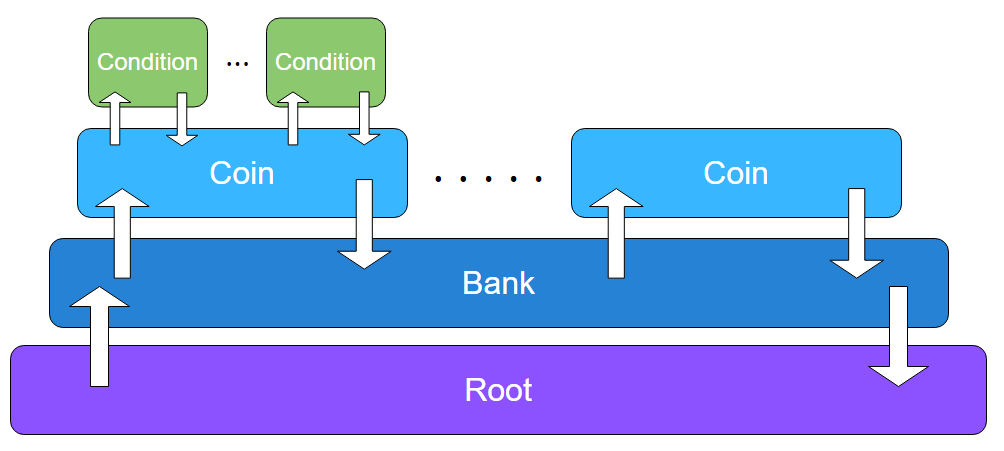
\includegraphics[scale=0.5]{figures/bank front end.PNG}  
    \caption{The flow of information through react components of the bank's front end}
    \label{fig:bankfront}
\end{figure}
What makes these components special is React's built-in rendering function. This function automatically re-renders a component should its state's contents be updated. This gives very responsive websites that allow for granular elements, as only changed elements need to be reloaded. These components are always called in another component resulting in a tree-like structure starting with the root component. Information getting directed towards the root usually denotes a function being called or information being aggregated. Information traveling towards child components usually serves to display information in the UI. These clear paths of information make React both quick and easy to develop with.\\
Fig 4.1 shows the existence of any number of coins being displayed in a bank. Any coin can also have a variable number of conditions. While a sponsorship contains more information than it's conditions, there is no reason to display this information using react components, as it is always of constant size.\\
\begin{figure}[H]
    \centering
    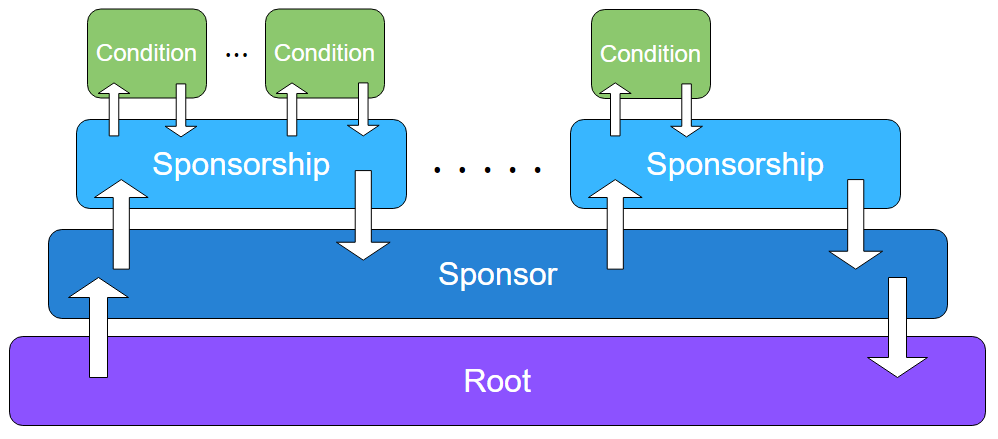
\includegraphics[scale=0.5]{figures/sponsor front end.PNG}  
    \caption{The flow of information through react components of Smart Sponsor's front end}
    \label{fig:sponsorfront}
\end{figure}
Finally, a large role of the front end is to clean inputs. Data given by users can be erroneous or incompatible with function parameters and causing unnecessary interactions with the blockchain can slow down performance or lead to unwanted transactions. At the same time, it is not advisable to ensure the input data's soundness in the back end, as this might cause unnecessary transactions to the blockchain. Therefore, the front end will be checking for empty string inputs, incorrect address formats, and input values that are guaranteed to run into reverts. To ensure security, these safeguards are for the most part also included in the back end, but these redundancies should ensure quicker responsiveness in the UI.\\
\\
A final decision that can be explored in a future extension of this application is Solidity's events. These events can inform the front end of certain transactions that have occurred. In this way, asynchronous processes, such as another user successfully applying for a sponsorship and then disappearing, could be updated without refreshing. This falls outside the scope of this prototype.
\section{Testing}
Testing has mainly been performed on the back end. The front end catches all errors thrown to ensure no crashes during runtime. The back end was tested on performance and has unit tests to ensure functionality throughout changes to the contracts' implementation.\\
\\
The unit tests over the smart contracts are fundamentally testing the limits of input parameters and ensuring the functions revert when they should. While the lower bound parameters of parameters are easily tested, the upper bounds are different. Solidity does not prevent or notify about integer overflows or underflows. In Smart Sponsors implementation, integer underflows cannot occur as there are no subtractions in any of the algorithms. On the other hand, integer overflows are possible. The identification numbers of Sponsor Coins and sponsorships are permanently increasing. Nonetheless, as those variables are \emph{uint256.} It is not likely that at any point there will be $2^{256}$ Sponsor Coins or sponsorships on the blockchain, so this can be disregarded. Still, should this ever pose a problem, OpenZeppelin offers a smart contract that implements checks to ensure no overflows occur\cite{Zeppelin}.\\
\\
All performance tests were done using a machine of the following specs and OS:
\begin{itemize}
    \item Processor: Intel(R) Core(TM) i5-6600 CPU @ 3.30GHz   3.30 GHz
    \item Graphics Processing Unit: NVIDIA GeForce GTX 970
    \item Motherboard: Gigabyte GA-B150-HD3P
    \item Random Access Memory: 16 GB (15,4 free)
    \item Operating System: Windows 10 Version 21H2 (OS Build 19044.1766)
\end{itemize}
All tests were run from the front-end client running on a simulated server and using the simulated blockchain Ganache\cite{truffle}. Every transaction that writes to the blockchain has a set amount of time it needs for MetaMask to establish the contract call, independently of the runtime of the contract. This time averages out to 3.16 seconds. This was established using a contract that only sets a boolean to true or false. This average time has not been subtracted from the results of the tests.\\
Algorithm 1 was tested with words of differing lengths. The time for the shortest input, a string of length 1, averaged 3.37 seconds while for a string of length 1500 the time rose to 3.41 seconds. It seems that due to the hashing algorithm the input length does not have a large factor in the performance.\\
Algorithm 2 was tested with different amounts of certificates. Attempting to update certificates if none are uploaded takes 3.32 seconds. After inserting 25 certificates this number rose to 3.41. It seems that every 25 active certificates add 0.1 seconds to this function call. If the number of active certificates rises higher, these calls need to be separated into different calls due to the limited block size.\\
\begin{figure}[H]
    \centering
    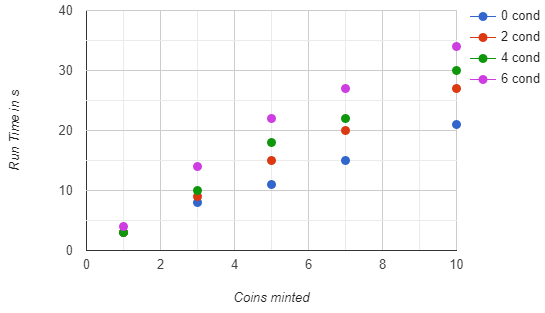
\includegraphics[scale=0.7]{figures/4.3.png}  
    \caption{Run times of algorithm 3 assuming differing amounts of conditions and currency}
    \label{fig:testalgo3}
\end{figure}
Algorithm 3 has 3 variables, the number of coins to mint, sender conditions, and receiver conditions. The latter act as the same, so for the tests they are grouped. Fig 4.3 shows these test results. While possible it seems unlikely to attach more than 6 conditions. At that point, it would be advisable to combine conditions as detailed for algorithm 3.\\
Algorithm 4 showed no substantial difference in increasing the number of coins to permit. For 1 coin the time was 3.9 seconds while for 10 it rose to 3.92 seconds. The maximum amount tested was 20 coins which were permitted after 3.95 seconds.\\
Algorithm 5 and algorithm 6 are shown in Fig 4.4. One sender condition and one receiver condition attached was assumed for the series outlined in the legend.
\begin{figure}[H]
    \centering
    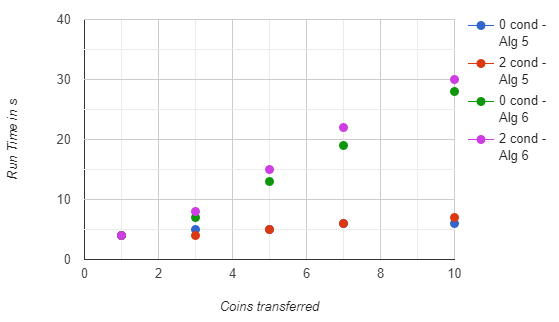
\includegraphics[scale=0.7]{figures/4.4.png}  
    \caption{Run times of algorithm 4 and 5 assuming 0 or 2 set conditions set to the transferred coins. Algorithm 6 attaches a sender and a receiver condition}
    \label{fig:testalgo56}
\end{figure}
It is observable that conditions being attached to a Sponsor Coin make a slight difference in run time. What has by far a larger impact is attaching new conditions. This follows the remarks outlined in the design decisions of algorithms 5 and 6.\\
Algorithms 7 and 8 mirror the numbers detailed in Fig 4.4. This is to be expected, as the centerpiece of these algorithms are the transaction methods. The setting of the sponsorship structure and testing if the applicant fulfills the conditions are a lot less computation-intensive.\\